\documentclass[12pt,a4paper]{article}
\topmargin -1.6cm
\addtolength{\textheight}{4cm}
\textwidth  15.5cm

\leftmargin      5mm
\rightmargin     5mm
\oddsidemargin   5mm
\evensidemargin  5mm

\usepackage{hyperref}
\usepackage{polski}
\usepackage[utf8]{inputenc}
\usepackage{graphicx}
\usepackage{units}
\usepackage{sty/style}
\usepackage{float}

\projekt{Modelowanie i identyfikacja}
\autor{Marcin Bober, 249426}
\przedmiot{Identyfikacja i modelowanie statystyczne}
\prowadzacy{Mgr inż. Maciej Filiński}

\begin{document}
\pdfpageheight   297mm
\pdfpagewidth    210mm

\StronaTytulowa
\SpisTresci

\pagebreak

% \section{Cel ćwiczenia}
%   Celem ćwiczenia jest zbadanie zachowania dwóch algorytmów sterowania sprzężonych z manipulatorem 2R. Mają one zrealizować zadanie śledzenia zadanej trajektorii.

\section{Generator liczb pseudolosowych}
  \subsection{Opis}
  Zadanie polega na implementacji generatora liczb pseudolosowych z rozkładu jednostajnego oraz analizie wyników uzyskanych z jego udziałem. Generator oparty jest na przekształceniu piłokształtnym o równaniu $X_{n+1} = X_n \cdot z - [X_n \cdot z]$ 

  \subsection{Wpływ wartości początkowej X na własności generatora}

  Wartość $Z$ ustawiona została na wartość 51. Wykorzystano 1000 próbek.

  \begin{figure}[H]
    \centering
    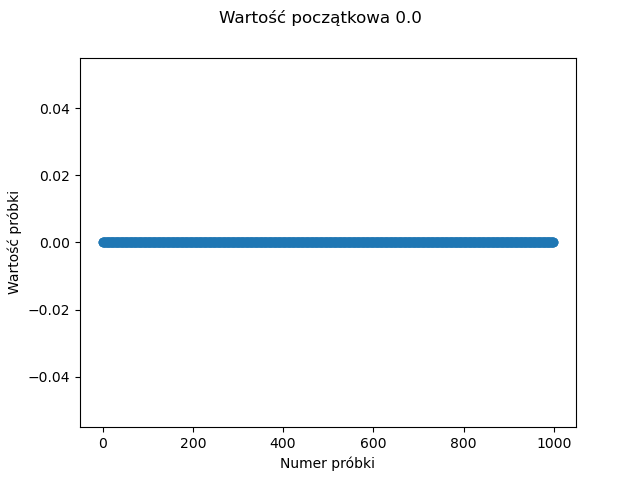
\includegraphics[height=0.3\textheight]{figures/Figure_1.png}
    \label{fig:1}
  \end{figure}

  \begin{figure}[H]
    \centering
    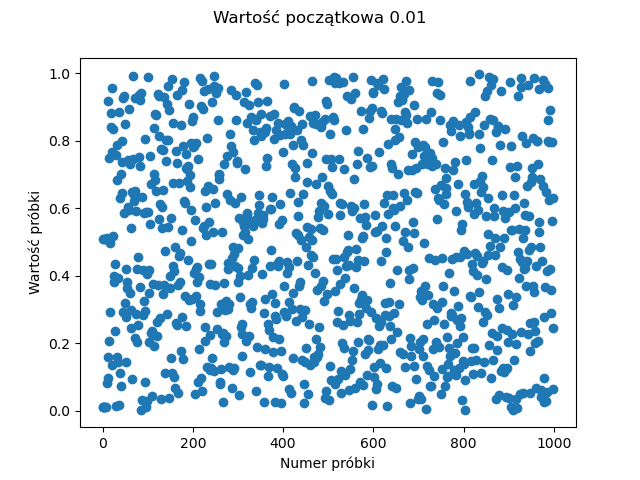
\includegraphics[height=0.3\textheight]{figures/Figure_2.png}
    \label{fig:2}
  \end{figure}

  \begin{figure}[H]
    \centering
    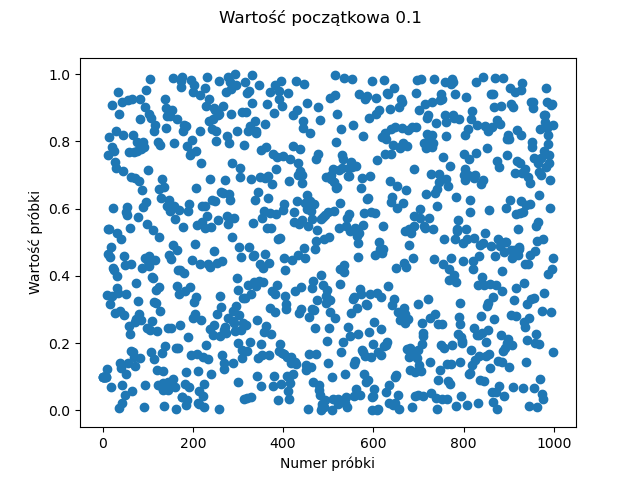
\includegraphics[height=0.3\textheight]{figures/Figure_3.png}
    \label{fig:3}
  \end{figure}

  \begin{figure}[H]
    \centering
    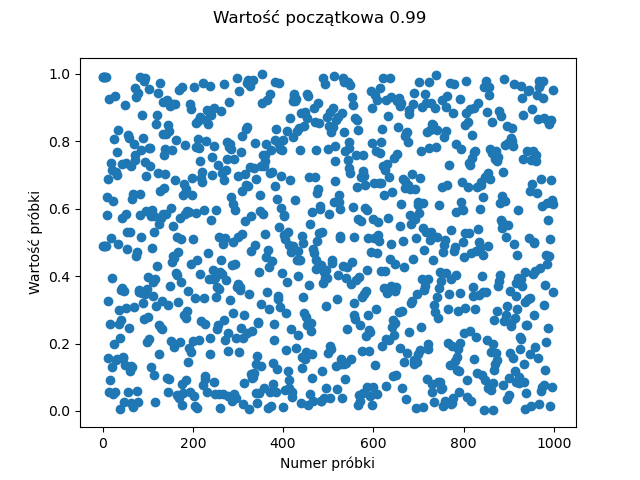
\includegraphics[height=0.3\textheight]{figures/Figure_4.png}
    \label{fig:4}
  \end{figure}

  \begin{figure}[H]
    \centering
    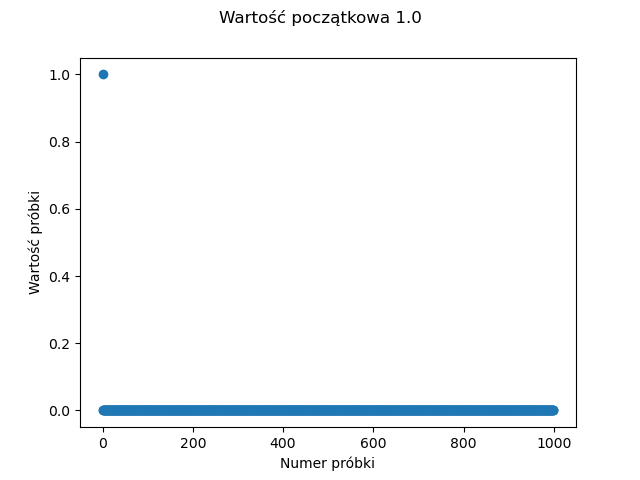
\includegraphics[height=0.3\textheight]{figures/Figure_5.png}
    \label{fig:5}
  \end{figure}
  
  \begin{itemize}
    \item Ustawienie wartości początkowej równej zero powoduje że wszystkie wygenerowane próbki są zerowe. (Patrz wykres \ref{fig:1}) Dzieje się tak ponieważ algorytm opiera się o obliczenie iloczynu liczb, których jednym ze składników jest zero.
    \item Wybór liczby całkowitej spowoduje że pierwsza próbka jest równa tej wartości, a wszystkie kolejne są zerowe (Patrz wykres \ref{fig:5}). Wynika to z faktu że obliczana jest reszta z dzielenia wartości przez jeden, która w taki wypadku zawsze równa jest zero.
    \item Zalecanym zakresem wyboru wartości początkowej jest przedział zawierający liczby większe od zera, z pominięciem liczb całkowitych.
  \end{itemize}

  \subsection{Wpływ parametru Z na własności generatora}

  Wartość $X_0$ ustawiona została na wartość 0,01. Wykorzystano 1000 próbek.

  \begin{figure}[H]
    \centering
    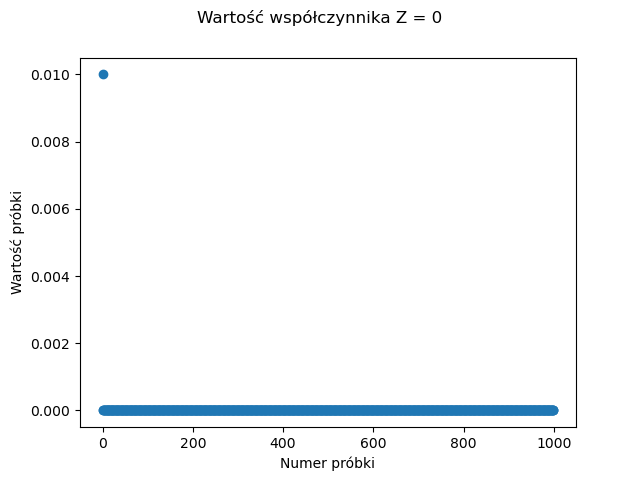
\includegraphics[height=0.3\textheight]{figures/Figure_6.png}
    \label{fig:6}
  \end{figure}

  \begin{figure}[H]
    \centering
    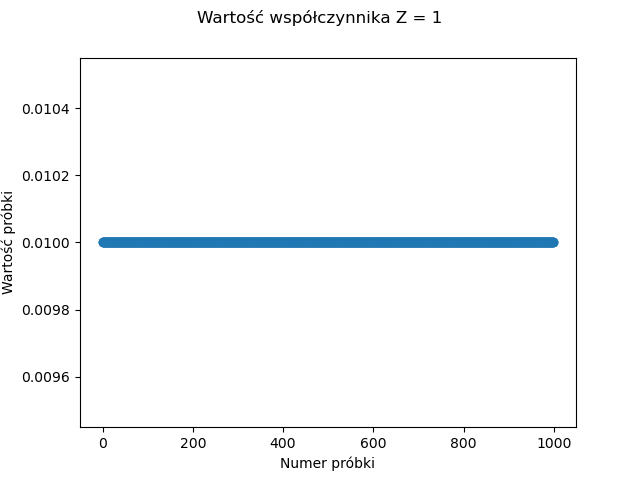
\includegraphics[height=0.3\textheight]{figures/Figure_7.png}
    \label{fig:7}
  \end{figure}

  \begin{figure}[H]
    \centering
    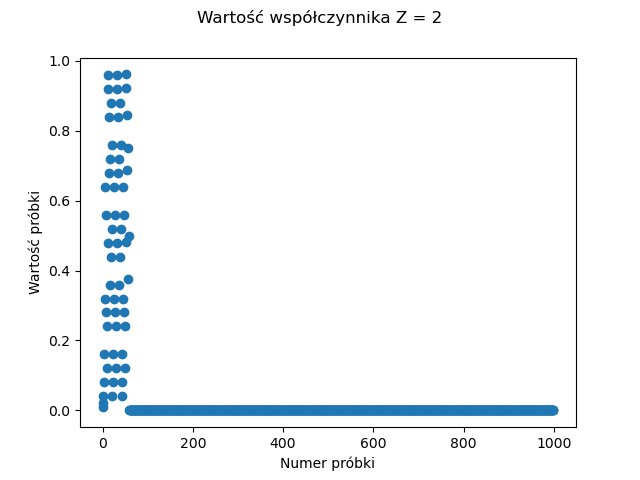
\includegraphics[height=0.3\textheight]{figures/Figure_8.png}
    \label{fig:8}
  \end{figure}

  \begin{figure}[H]
    \centering
    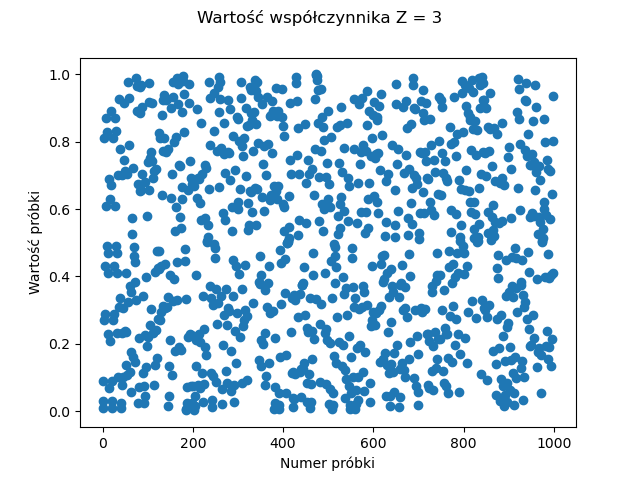
\includegraphics[height=0.3\textheight]{figures/Figure_9.png}
    \label{fig:9}
  \end{figure}
  
  \begin{itemize}
    \item Dla zerowego współczynnika $Z$ pierwsza próbka uzyskuje wartość początkowa, a kolejne są zerami. Wynika to z mnożenia tych wyników przez współczynnik $Z$ czyli zero.
    \item Gdy wartość $Z$ jest równa jedności, wszystkie otrzymane wyniki są identyczne z wartością startową.
    \item W przypadku wykorzystania liczb parzystych, uzyskiwane wyniki szybko trafiają na wartość zero, która powoduje zatrzymanie generowania kolejnych wartości losowych. 
    \item Najlepsze wyniki otrzymywane są dla współczynnika $Z$ będącego dużą liczbą pierwszą. 
  \end{itemize}

  \subsection{Okres generatora dla wybranych wartości Z}

  \begin{table}[h!]
    \centering
    \begin{tabular}{ c | c | c }
      $X_0$ & $Z$ & okres generatora  \\ 
      \hline
      0,1 & 1 & 1  \\  
      0,1 & 2 & 4  \\  
      0,1 & 3 & 4  \\  
      0,1 & 4 & 2  \\  
      0,1 & 5 & 1  \\
      0,1 & 6 & 1  \\
      0,1 & 7 & 4  \\
      0,1 & 8 & 4 
    \end{tabular}
    \caption{Nastawy PD i odpowiadający im rząd błędu.}
    \label{table:1}
  \end{table}

  \subsection{Podobieństwo histogramu ciągu wygenerowaych liczb, a gęstość rozkładu jednostajnego}


  \begin{figure}[H]
    \centering
    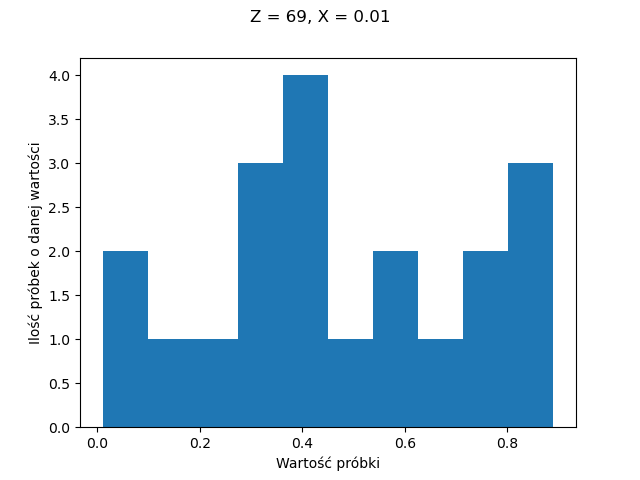
\includegraphics[height=0.25\textheight]{figures/Figure_10.png}
    \caption{Ilość wygenerowanych próbek - 20}
    \label{fig:10}
  \end{figure}

  \begin{figure}[H]
    \centering
    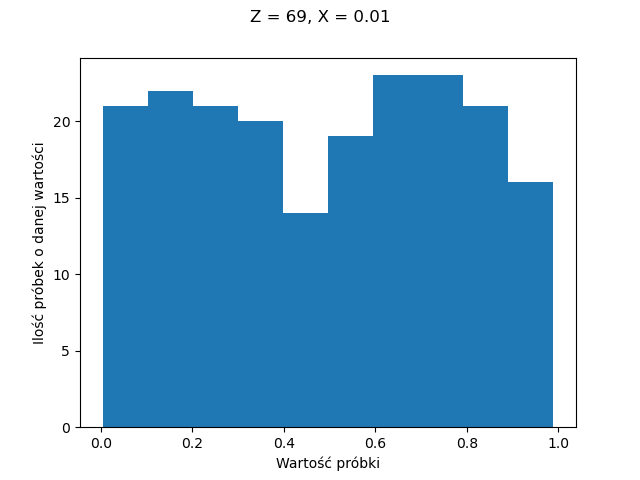
\includegraphics[height=0.25\textheight]{figures/Figure_11.png}
    \caption{Ilość wygenerowanych próbek - 200}
    \label{fig:11}
  \end{figure}

  \begin{figure}[H]
    \centering
    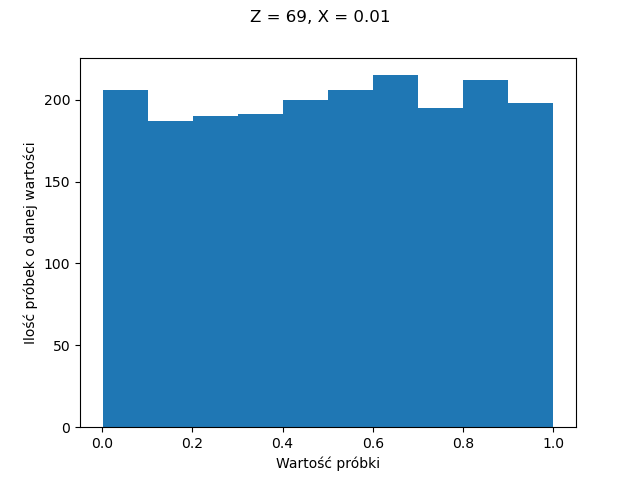
\includegraphics[height=0.25\textheight]{figures/Figure_12.png}
    \caption{Ilość wygenerowanych próbek - 2000}
    \label{fig:12}
  \end{figure}

  \begin{figure}[H]
    \centering
    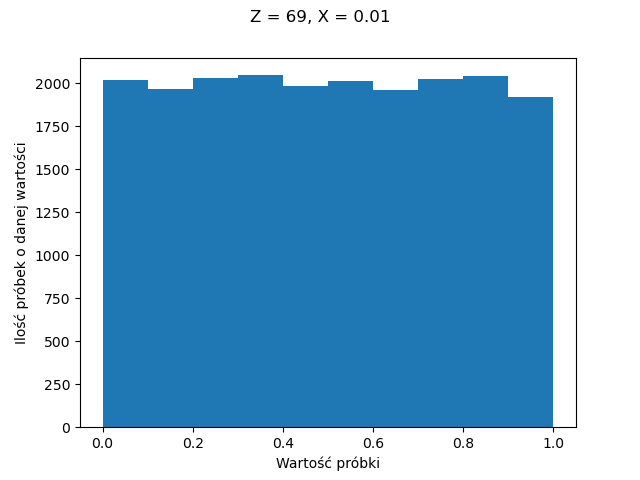
\includegraphics[height=0.25\textheight]{figures/Figure_13.png}
    \caption{Ilość wygenerowanych próbek - 20000}
    \label{fig:13}
  \end{figure}


    % Algorytm Qui Dorsey'a jest algorytmem globalnym. Jego zasada działania jest tożsama z działaniem liniowego regulatora PD. Z powodu liniowej natury algorytmu i nieliniowego charakteru obiektu, sterowanie obiektem nie będzie proste. W celu zbadania właściwości nastaw regulatora na błąd śledzenia trajektorii (uchyb) został przeprowadzony szereg symulacji. Przetestowane nastawy wraz z rzędem błędu sterowania zostały podane w tabeli \ref{table:1}.

  % \subsection{Wyniki} %tabelka - zmiany nastaw a rząd błędu
    % W tabeli \ref{table:1} znajduje się zestaw siedmiu par nastaw dla KP i KD regulatora. W kolejnych kolumnach został umieszczony rząd błędu sterowania odpowiadający podany parametrom. 




%   \begin{figure}[H]
%     \centering
%     \includegraphics[height=0.4\textheight]{figures/qui10.jpg}
%     \caption{KP = 10, KD = 1}
%     \label{fig:10}
%   \end{figure}

%     Niewielkie nastawy sprawiają że obiekt ma znaczne problemy ze śledzeniem zadanej trajektorii. Błąd śledzenia dla  KP = 10 i KD = 1 w zależności do czasu został zaprezentowany na rysunku \ref{fig:10}.

%   \begin{figure}[H]
%     \centering
%     \includegraphics[height=0.4\textheight]{figures/qui100.jpg}
%     \caption{KP = 100, KD = 10}
%     \label{fig:100}
%   \end{figure}

%     Konsekwentne zwiększanie nastaw regulatora przynosi wymierne efekty w postaci malejącego błędu. Można je zaobserwować porównująć wykresy \ref{fig:1000} oraz \ref{fig:10000}. 

%   \begin{figure}[H]
%     \centering
%     \includegraphics[height=0.4\textheight]{figures/qui1000.jpg}
%     \caption{KP = 1000, KD = 100}
%     \label{fig:1000}
%   \end{figure}


%   \begin{figure}[H]
%     \centering
%     \includegraphics[height=0.4\textheight]{figures/qui10000.jpg}
%     \caption{KP = 10000, KD = 1000}
%     \label{fig:10000}
%   \end{figure}

%     Pomimo malejącego błedu należy zaznaczyć że uzyskane przebiegi w każdej iteracji posiadają charakter niegasnących oscylacji. Jest to dobrze widoczne na rysunku \ref{fig:10000000}, gdzie błąd rzędu $10^{-6}$ wciąż oscyluje.

%   \begin{figure}[H]
%     \centering
%     \includegraphics[height=0.45\textheight]{figures/qui10000000_2.jpg}
%     \caption{KP = 10000000, KD = 1000000}
%     \label{fig:10000000}
%   \end{figure}

%     Stosowanie coraz to większych parametrów regulatora PD powoduje znaczący wzrost złożoności obliczeniowej.

%   \subsection{Wnioski}
%     Symulacje wykazały że algorytm realizuje cel minimalizacji błędu śledzenia dokładniej w przypadku zastosowania większych nastaw. Jednakże osiągnięcie zerowego błędu nie jest możliwe ponieważ wymagałoby ono nieskończonej wartości nastaw. W każdym zbadanym przypadku przebiegi błędów mają charakter niegasnących oscylacji.


% \section{Algorytm dokładnej linearyzacji}
%   \subsection{Opis} %(algorytmu i obiektu)
%     Algorym dokładnej linearyzacji może być zastosowany jedynie dla obiektów w pełni znanych. Niezbędne jest przeprowadzenie linearyzacji statycznej w celu otrzymania układu liniowego podówjego integratora.
%   \subsection{Zależność od wzmocnienia K0}
%     Symulacje przeprowadzono przy stałym wzmocnieniu K1 wynoszącym 1 oraz zmianie parametru K0.

%     \begin{figure}[H]
%       \centering
%       \includegraphics[width=1\textwidth]{figures/lin1.jpg}
%       \caption{stałe K1 = 1, zmienne K0}
%       \label{fig:lin1}
%     \end{figure}

%     \begin{table}[h!]
%       \centering
%       \begin{tabular}{ r | c | c }
%         K0 & Przesterowanie $e_1$ [rad] & Przesterowanie $e_2$ [rad] \\ 
%         \hline
%         1 & 0.16 & 0.33  \\
%         10 & 1.08 & 21.36   \\
%         20 & 1.66 & 49.91
%       \end{tabular}
%       \caption{Przesterowanie przebiegów w zależności od K0.}
%       \label{table:2}
%     \end{table}

%       Według tabeli \ref{table:2} wraz ze wzrostem wzmocnienia K0 wzrasta przesterowanie.

%     \begin{table}[h!]
%       \centering
%       \begin{tabular}{ r | c | c }
%         K0 & Czas wygaszania $e_1$ [s] & Czas wygaszania $e_2$ [s]  \\ 
%         \hline
%         1  &  8 & 7 \\
%         10 & 15 & 13  \\
%         20 & 20 & 15
%       \end{tabular}
%       \caption{Czas wygaszania przebiegów w zależności od K0.}
%       \label{table:3}
%     \end{table}

%       Według tabeli \ref{table:3} wraz ze wzrostem wzmocnienia K0 wydłuża się czas wygaszania oscylacji.




%   \subsection{Zależność od wzmocnienia K1}
%   Symulacje przeprowadzono przy stałym wzmocnieniu K0 wynoszącym 1 oraz zmianie parametru K1.

%   \begin{figure}[H]
%     \centering
%     \includegraphics[width=1\textwidth]{figures/lin2.jpg}
%     \caption{stałe K0 = 1, zmienne K1}
%     \label{fig:lin2}
%   \end{figure}

%   \begin{table}[h!]
%     \centering
%     \begin{tabular}{ r | c | c }
%       K1 & Przesterowanie $e_1$ [rad] & Czas wygaszania $e_1$ \\ 
%       \hline
%       1 & $15.87 \cdot 10^{-2}$ & 8  \\
%       5 & $4.52  \cdot 10^{-2}$ & 12   \\
%       9 & $2.64  \cdot 10^{-2}$ & 16
%     \end{tabular}
%     \caption{Charakterystyka przebiegów błędu $e_1$ w zależności od K1.}
%     \label{table:4}
%   \end{table}

%     Wzrost wzmocnienia K1 powoduje spadek przesterowania przegubu pierwszego. Negatywnym skutkiem takich nastaw jest wydłużony czas wygaszania oscylacji (patrz tabela \ref{table:4}).

%   \begin{table}[h!]
%     \centering
%     \begin{tabular}{ r | c | c }
%       K1 & Przesterowanie $e_2$ [rad] & Czas wygaszania $e_2$ [s]  \\ 
%       \hline
%       1 & $37.8 \cdot 10^{-2}$ & 12 \\
%       2 & $1.41 \cdot 10^{-6}$ & 8  \\
%       3 & $2.36 \cdot 10^{-3}$ & 15
%     \end{tabular}
%     \caption{Charakterystyka przebiegów błędu $e_2$ w zależności od K1.}
%     \label{table:5}
%   \end{table}

%     Najlepsze zachowanie przegubu drugiego zaobserwowano dla wzmocnienia $K1=2$ (patrz tabela \ref{table:5}).


%   \subsection{Zależność od wartości początkowej}

%     Rysunek \ref{fig:lin3} przedstawia przebiegi błędów śledzenia trajektorii w zależności od różnych punktów startowych.

%   \begin{figure}[H]
%     \centering
%     \includegraphics[width=1\textwidth]{figures/lin3.jpg}
%     \caption{Charakterystyka przebiegów błędu w zależności od położenia początkowego.}
%     \label{fig:lin3}
%   \end{figure}

%     Pierwsza część wykresu \ref{fig:lin3} dotyczy zmiany położenia pierwszego przegubu. Im przegub startuje z miejsca bardziej oddalonego od punktu zerowego tym większy błąd początkowy i dłuższy czas stabilizacji. Druga część wykresu odpowiada za drugi przegób. W tym przypadku również większe wychylenia powodują identyczne skutki, jak w pierwszym przegubie.

%   \begin{figure}[H]
%     \centering
%     \includegraphics[width=1\textwidth]{figures/lin4.jpg}
%     \caption{Charakterystyka przebiegów błędu w zależności od prędkości początkowej.}
%     \label{fig:lin4}
%   \end{figure}

%     Wykres \ref{fig:lin4} prezentuje jaki wpływ na błąd śledzenia ma prędkość początkowa. W górnej części poświęconej przegubowi pierwszemu, zwiększanie prędkości początkowej powoduje coraz to większe przesterowania. Dolna część dotycząca drugiego przegubu przy pewnej prędkości początkowej ma dużo mniejszy błąd niż przy starcie ze stanu spoczynku. Jest to spowodowane tym że odpowiednio rozpędzony przegób może szybciej znaleźć się w zadanym położeniu. Intuicyjne jest również to że przy zbyt wielkiej prędkości błąd znów zacznie rosnąć. 

  % \subsection{Wnioski}

%   \begin{itemize}
%     \item wzrost wzmocnienia K0 powoduje zwiększone przesterowanie i wydłużony czas tłumienia oscylacji dla obu przegubów,
%     \item wzrost wzmocnienia K1 powoduje spadek przesterowania i wydłużony czas tłumienia oscylacji dla przegubu pierwszego,
%     \item dla przegubu drugiego ustawienie wzmocnienienia $K1=2$ spowodowało osiągnięcie najlepszych rezultatów,
%     \item położenie i prędkość początkowa mają duże znaczenie na błąd w pierwszych sekundach sterowania. 
%   \end{itemize}
  
\section{Podsumowanie}
%   Algorytm Qui Dorsey’a jest prostrzy w implementacji. Poza tym jest on algorytmem globalnym co sprawia że powinien działać on przy każdych wartościach początkowych. Do jego wad należy słaba jakość sterowania, ponieważ błąd śledzenia wiecznie oscyluje. Co więcej, jest on obarczony dużo większą złożonością obliczeniową. Zwiększanie nastaw w nieskończoność powoduje minimalizację błędu.

%   Algorytm dokładnej linearyzacji dużo lepiej radzi sobie z osiągnięciem zadanej trajektorii. Jest on dużo dokładniejszy pomimo faktu że jest znacznie mniej obciążający obliczeniowo. Zwiększanie wzmocnienia w nieskończoność nie powoduje minimalizacji błędu.

\end{document}